\documentclass{article}

\usepackage[T1]{fontenc}
\usepackage[utf8]{inputenc}
\usepackage{amsmath, amsfonts}
\usepackage{graphicx, color}
\usepackage{lmodern}
\usepackage{microtype}

\author{Axel Forsman}
\title{TMA372 Assignment 2}

\begin{document}
\maketitle

\section{Theoretical Part}

We consider the linear heat equation

\begin{align*}
  u_t(x) - \Delta u(x) &= 0, \quad x \in \Omega, t > 0 \\
  u(x, t) &= 0, \quad x \in \partial\Omega, t > 0 \\
  u(x, 0) &= u_0(x), \quad x \in \Omega
\end{align*}

\subsection{(a)}

We find the following variational formulation:
\begin{equation*}
  \text{Find $u \in V = H_0^1(\Omega)$ st. } (u_t, v)_{L^2} + (\nabla u, \nabla v)_{L^2} = 0
  \quad \forall v \in V \tag{VF}
\end{equation*}
To show the first stability estimate we test against $u$:
$$ (u_t, u) + (\nabla u, \nabla u) = 0 $$
where the first term can be rewritten as $\frac12 \frac d{dt} \lVert u(\cdot, t) \rVert_{L^2}^2$,
and the second term as $\lVert \nabla u(\cdot, t) \rVert_{L^2}^2$
using Green's formula and the fact that $u$ is zero on the boundary.
Then, if we integrate in time $\int_0^t \cdots \, dt$ we get
$$ \lVert u(\cdot, t) \rVert_{L^2}^2 - \lVert u_0 \rVert_{L^2}^2 + 2 \int_0^t \lVert \nabla u(\cdot, s) \rVert_{L^2}^2 \, ds = 0 $$
where the integral can be shown to be non-negative using
triangle inequality for integrals and the properties of the norm,
which proves the first estimate.

For the the second estimate we multiply the differential equation
by $t^2 \Delta^2 u$ following the hint by Asadzadeh
$$ t^2 \int_\Omega u_t \Delta^2 u \, dx - t^2 \int_\Omega \Delta^2 u \Delta u \, dx = 0 $$
and note that the first integral can be written
\begin{equation*}
  \int_\Omega u_t \Delta^2 u \, dx = \int_\Omega \Delta u \Delta (u_t) \, dx
  = \int_\Omega \frac12 \frac d{dt} (\Delta u)^2 = \frac12 \frac d{dt} \lVert \Delta u \rVert_{L^2}^2
\end{equation*}
since $u_t = \Delta u$.
Next we use that
$\frac12 \frac d{dt} (t^2 \lVert \Delta u \rVert^2) = t \lVert \Delta u \rVert^2 + t^2 \frac12 \frac d{dt} \lVert \Delta u \rVert^2$
to write the previous equation as
$$ \frac12 \frac d{dt} (t^2 \lVert \Delta u \rVert^2) - t^2 \int_\Omega \Delta^2 u \Delta u \, dx = t \lVert \Delta u \rVert^2 $$
Integrating in time $\int_0^t \cdots \, dt$ yields
$$ \frac12 t^2 \lVert \Delta u \rVert^2 - \int_0^t t^2 \int_\Omega \Delta^2 u \Delta u \, dx dt = \int_0^t t \lVert \Delta u \rVert^2 \le \frac14 \lVert u_0 \rVert^2 $$
where the inequality is due to equation (10.1.14) in the book.
Since, using Green's formula,
$$ \int_\Omega \Delta^2 u \Delta u \, dx = -\lVert \nabla \Delta u \rVert^2 \le 0 $$
we can remove the integral term from the above inequality.
Taking the square root of both sides and dividing by $t$,
we obtain the wanted estimate.

\subsection{(b)}

To investigate how the estimates would look like
with $\Delta$ replaced by the operator
$\widetilde\Delta = \frac{\partial^2}{\partial x_1^2} + 4 \frac{\partial^2}{\partial x_2^2}$,
we note that $\widetilde\Delta u = \Delta u + 3 u_{x_2 x_2}$.
Therefore for the first estimate,
due to linearity, in the new variational formulation
we only have to add the additional new term
$$ -\int_\Omega u \, 3 u_{x_2 x_2} \, dx = 3 \int_\Omega u_{x_2}^2 \, dx = \lVert u_{x_2} \rVert_{L^2}^2 $$
where we used integration by parts for the first equality.
Therefore, repeating the same steps, the new first estimate becomes
$$ \lVert u(\cdot, t) \rVert_{L^2}^2 + \int_0^t \left( \lVert \nabla u(\cdot, s) \rVert_{L^2}^2 + 3 \lVert u_{x_2} \rVert_{L^2}^2 \right) \, ds \le \lVert u_0 \rVert_{L^2}^2 $$

Then for the second estimate we repeat the exact same steps
except replacing $\Delta$ by $\widetilde\Delta$.
As before $\int_\Omega \widetilde\Delta^2 u \widetilde\Delta u \, dx$
can be shown to be negative, again using partial integration.
We end up with the new estimate
$$ \lVert \widetilde\Delta u \rVert \le \frac1t \lVert u_0 \rVert $$

\subsection{(c)}

To derive a Fourier series for the solution in the case $\Omega = [0, 1]$
we use separation of variables with the ansats $u = X(x)T(t)$.
Substitution into the DE gives
$$ \frac{T'}T = \frac{X''}X = \text{const} = \lambda $$
since the respective expressions are invariant of $x, t$.
Starting with $X$, the differential equation
$$ X'' - \lambda X = 0 $$
only has nontrivial solutions for the case $\lambda<0$,
in which case the solution for the particular boundary conditions is
$$ X_n = a_n \sin(\pi n x), \quad \lambda_n = -\pi^2 n^2 \quad n \in \mathrm N_0 $$
Solving for $T$ we get $T_n = e^{-\pi^2 n^2 t}$ up to a constant.
The superposition principle gives use the solution $u$ to the heat equation
$$ u(x, t) = \sum_{n \ge 0} a_n \sin(\pi n x) e^{-\pi^2 n^2 t} $$
To accomodate the initial condition we let $u(x, 0)$
be the $L^2$-projection of $u_0$ onto the $\sin(\pi n x)$ basis vectors:
$$ a_n = \frac1{\lVert \sin(\pi n x) \rVert^2} (u_0, \sin(\pi n x))_{L^2} $$

A result from Fourier analysis is that the Fourier coefficients
decay as $1/n^k$ if $u_0 \in C^k$.
We can show this using partial integration
\begin{align*}
  a_n &\propto \int_0^1 u_0(t) \sin(\pi n t) \, dt
  = \left. u_0(t) \frac{-1}{\pi n} \cos(\pi n t) \right\vert_0^1
  + \frac1{\pi n} \int_0^1 u_0'(t) \cos(\pi n t) \, dt \\
  &\propto \frac1n \int_0^1 u_0'(t) \cos(\pi n t) \, dt
\end{align*}
where $\int_0^1 u_0'(t) \cos(\pi n t) \, dt$
tends to $0$ as $n \to \infty$ per the Riemann-Lebesgue lemma.

We can now show the smoothing estimate using the Fourier series solution
\begin{align*}
  t \lVert \Delta u(x, t) \rVert &= \lVert \sum_{n \ge 0} a_n \sin{\pi n x} \pi^2 n^2 t e^{-\pi^2 n^2 t} \rVert \\
  \le \lVert \sum_{n \ge 0} a_n \sin{\pi n x} \rVert = \lVert u_0 \rVert
\end{align*}
where we have used that $x e^{-x} < 1$ for all $x \ge 0$.

\section{Non Theoretical Part}

We consider the problem of 2d incompressible irrotational fluid flow
through a nozzle.
Nozzles are in widespread use for modulating both
fluid velocity and direction.
As the cross sectional area of a nozzle shrinks
the velocity of a passing fluid increases
at the expense of decreased pressure.
Take for instance the manufacturing of nozzles for spray guns.
For this purpose it is important to understand how the nozzle
will influence the spray,
and also how possible defects in production can
end up affecting the use of the product.

Let $u=(u_x, u_y)$ be the fluid velocity.
The irrotationality property ensures the existence of a
scalar potential $\phi$ such that $u = \nabla\phi$,
and the incompressibility requirement, $\nabla \cdot u = 0$,
gives the Laplace equation for $\phi$
$$ \Delta\phi = 0 $$
Together with the boundary conditions that define the inlet and walls
of the domain $\Omega$, see figure~\ref{fig:domain},
we get our PDE
\begin{equation*}
  \left\{ \begin{aligned}
    \Delta\phi &= 0 \quad x \in \Omega \\
    \hat n \cdot \nabla\phi &= g \quad x \in \Gamma_1, g \in \mathrm R \\
    \hat n \cdot \nabla\phi &= 0 \quad x \in \Gamma_2 \\
    \phi &= 0 \quad x \in \Gamma_3
    \end{aligned} \right.
\end{equation*}
where $g$ is the velocity of the fluid entering the nozzle,
and the last BC pins an arbitrary reference potential.

\begin{figure}
  \centering
  \def\svgwidth{0.6\linewidth}
  \input{domain.pdf_tex}
  \caption{The domain we will consider of the fluid flowing through the nozzle. \label{fig:domain}}
\end{figure}

In order to derive a variational formulation we multiply by
a test function $v \in V = \{v \in H^1(\Omega): v(\Gamma_3) = 0\}$
and integrate
$$ \int_\Omega \Delta\phi v \, dx = \int_{\partial\Omega} (\hat n \cdot \nabla \phi) v \, dx - \int_\Omega \nabla\phi \cdot \nabla v \, dx = 0 $$
where we used Green's formula.
We get the variational formulation
\begin{equation*}
  \text{Find $\phi \in V$ st. } (\nabla\phi, \nabla v) = g \int_{\Gamma_1} v \, dx \quad \forall v \in V
\end{equation*}
Now, given a suitable triangulation $T_h = \{K\}$ of $\Omega$ we define 
the finite dimensional space
$V_h = \{v \in V: \text{$v$ cont. pw. linear on $T_h$}\}$,
which can be constructed as the span of shape functions $\varphi_i$
where we include the half shape functions centered on exterior points
$x_p \notin \Gamma_3$.
The FE problem then becomes
\begin{equation*}
  \text{Find $\phi_h \in V_h$ st. } (\nabla\phi_h, \nabla \chi) = g \int_{\Gamma_1} \chi \, dx \quad \forall \chi \in V_h
\end{equation*}
To get a linear system we choose $\chi = \varphi_i$
and write $\phi_h = \sum_j \zeta_j \varphi_j(x)$:
$$ S \zeta = b $$
where $S$ is the stiffness matrix,
with entries $S_{ij} = \int_\Omega \nabla\varphi_i \cdot \nabla\varphi_j \, dx$,
and $b$ is a vector with entries
$b_i = g \int_{\Gamma_1} \varphi \, dx$.

The numerical solution to the model obtained by using MATLAB's PDE Modeler
is shown in figure~\ref{fig:pde-sol}.
We see that as one would expect the fluid velocity increases
as it is compressed through the nozzle,
before quickly dissipating once it has exited.

\begin{figure}
  \centering
  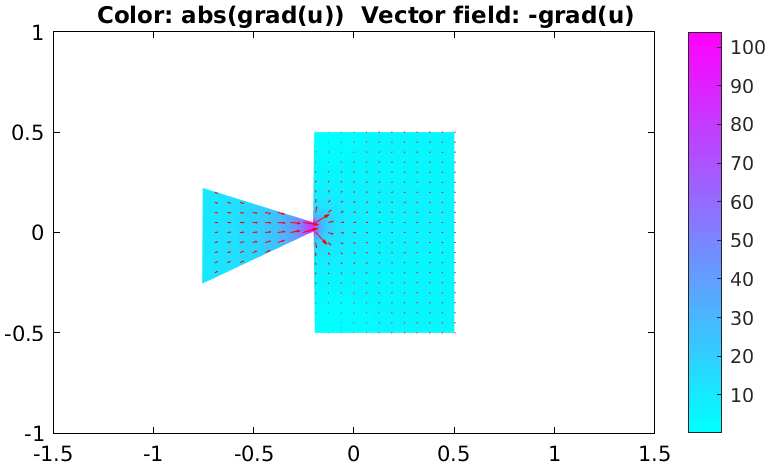
\includegraphics[width=\textwidth]{pde-sol}
  \caption{Numerical solution $\phi_h$ computed using MATLAB's PDE Modeler. \label{fig:pde-sol}}
\end{figure}

\subsection{Simplified Model}

If we instead look at homogeneous Dirichlet boundary conditions
for the whole boundary $\partial\Omega$ of the domain,
noting that Laplace's equation is a special case
of Poisson's equation with the right-hand side being zero,
we can apply the a posteriori error estimate given
in the course book as theorem 11.5, which says that
$$ \lVert \phi - \phi_h \rVert \le C \lVert h^2 \Delta_h \phi_h \rVert $$
where $h$ is the maximum diameter of any triangle element $K \in T_h$
and $\Delta_h$ is the discrete Laplacian on $T_h$.

If we allow allow ourselves to constrain our model
to use a simplified domain, see figure~\ref{fig:simple-domain},
we can give an explicit solution.
Consider the simplified model
\begin{equation*}
  \left\{ \begin{aligned}
    \Delta\phi &= 0 \quad x \in \Omega \\
    \frac{\partial\phi}{\partial x} &= g \quad x \in \Gamma_1 \\
    \frac{\partial\phi}{\partial y} &= 0 \quad x \in \Gamma_2 \cup \Gamma_4 \\
    \phi &= 0 \quad x \in \Gamma_3
    \end{aligned} \right.
\end{equation*}
While otherwise accurate, in this simpler model
the nozzle is not much of a nozzle anymore.
Here $\phi = g x$ will be a solution to the PDE,
representing a straight laminar flow,
which is rather uninteresting.
It is easy to see that we will then have
$$ \lVert u \rVert = \lVert \nabla\phi \rVert = g $$
that is, the fluid velocity is constant throughout.

\begin{figure}
  \centering
  \def\svgwidth{0.6\linewidth}
  \input{simple-model.pdf_tex}
  \caption{Simple model with a simplified domain. \label{fig:simple-domain}}
\end{figure}

\end{document}
